%%%%%%%%%%%%%%%%%%%%%%%%%%%%%%%%%%%%%%%%%%%%%%%%%%%%%%%%%%%%%%%%%%
\chapter{\SOCA}

\todo{what is software cartography, how do we do it }

% =============================================================================
\section{On the Choice of Vocabulary}

The decision to use a distance based on lexical similarity does, indeed, create a distribution of distances that should not change a lot in time. This is because programmers will not use a completely new set of lexical tokens in each new version of the software. In fact, it has been shown that over time vocabulary tends to be more stable than the structure of software \cite{Anto07a}. However, this also will create software maps that naturally only can show how items are similar from a lexical point of view.

The map layout as presented in this work can, of course, be used to see how items are related from the point of view of some other distance, such as considering structural similarity, similarity with regard to a complexity or testability metric. In that case, the distance may vary a lot over time during the evolution of a product, and this will create unstable layouts. The focus of this work, however, is the creation of maps that help programmers to establish a stable mental model of their software system under work. In any case, if maps  based on other metrics are ever to be used in conjunction with vocabulary-based \SOCA maps, we strongly recommend to visually distinguish them by using another rendering scheme. This helps to reduce the likeliness that programmers confuse the spatial layout of these other maps, with the mental model acquired through the use of \SOCA maps. 

As mentioned in the introduction, \SOCA is vocabulary-based because vocabulary can effectively \emph{abstract} away from the technical details of source code \cite{Kuhn07a} by capturing the key domain concepts of source code. The assumption being that software entities with similar vocabulary are conceptually and topically close. Consider, for example, programming languages and software where name overloading is applied. Even though overloaded methods differ in their implementation strategy, they will typically implement the same concept using the same vocabulary. In fact, lexical similarity has proven useful to detect high-level clones \cite{Marc01a} and cross-cutting concerns \cite{Pali08a} in software.  

Due to name scoping, semantically different scopes can have identical names with different meanings. Consider, for example, two large functions having mostly identifiers such as i, j, prev, next, end, stop, flag, \dots;  the one does some matrix computations, while the other is a hash-table implementation. Without the application of \LSI (\secref{lsi}) the two would be classified as being very similar, while this is clearly not true from a developer's perspective. \LSI, however, can identify words that have different meaning depending on their context. LSI has the ability to resolve certain synonymy and polysemy \cite{Deer90a}.


Although refactorings may cause functionality to be renamed or moved, the overall vocabulary tends not to change, except as a side-effect of growth \cite{Zhan08a,Vasa07b}. Consider the example of a rename refactoring. Two effects may occur. 
In the first case, all occurrences of a symbol are replaced with new symbol. This will not affect the map, since both lexical similarity and LSI are based on statistical analysis only. Replacing all occurrences of one term with a new term is, from the point of these IR technologies, a null operation. In the second case, some occurrences of a symbol are replaced with another symbol which is already used. This will indeed affect the layout of the map. Given that the new name was well chosen by the programmer, the new layout constitutes a better representation of the system. On the other hand, if the new name is a bad choice, the new layout is flawed. However, what constitutes bad naming is not merely a matter of taste. Approaches that combine vocabulary with structural information can indeed assess the quality of naming. Please refer to H\o{}st's recent work on debugging method names for further reading \cite{Hoes09a}.

Not considered in the present work is the relative weight of different lexical tokens. For example, it seems reasonable to weight local identifiers differently than identifiers in top-level namespaces. Also, one may treat names coming from library functions different from the ones coming from the actual user code. Given the absence of evaluation benchmarks, we decided to use equal weighting for all lexical token. Also, preliminary experiments with different weighting schemes indicate that relative weights below boost level, \ie below a factor of 10, do often not significantly affect the overall layout.

In this section we present the techniques that are used to achieve a consistent layout for software maps. We present two variations of \SOCA, an \emph{offline} algorithm that requires that all releases of a software system are available upfront, and an improved \emph{online} algorithm that updates the layout incrementally as new releases of the system appear. 

The general approach of \SOCA, as illustrated in \autoref{fig:soca}, is as follows:
\begin{enumerate}
\item We parse the vocabulary of source files into term-frequency histograms. All text found in raw source code is taken into account, including not only identifiers but also comments and literals.
\item We transform the term-frequency histograms using \LSI (LSI) \cite{Deer90a}, an information retrieval technique that resolves synonymy and polysemy. 
\item We use \MDS (MDS) \cite{Borg05a} to map the term-frequency histograms onto the 2D visualization pane. This preserves the lexical co-relation of source files as well as possible.
\item We use cartographic visualization techniques to render an aesthetically appealing landscape.
\end{enumerate}

Possible applications of \SOCA in the software development process are, \dots

\begin{itemize}
\item \dots to navigate within a software system, be it for development or analysis.
\item \dots to relate different metrics to each other, \eg search results and bug prediction.
\item \dots to stay in touch with other developers of your team, by showing open files of other developers.
\item \dots to understand a system’s domain upon first contact.
\item \dots to explore a system during reverse engineering.
\end{itemize}

\noindent We implemented a prototype of our approach, \TOOL, which is available as an open source project. \TOOL was originally programmed in Smalltalk, in the mean time development has been moved to Java. \TOOL is available as an Eclipse plug-in\footnote{\url{http://scg.unibe.ch/codemap}}.

% =============================================================================
\section{Implementation}

% ~~~~~~~~~~~~~~~~~~~~~~~~~~~~~~~~~~~~~~~~~~~~~~~~~~~~~~~~~~~~~~~~~~~~~~~~~~~~~
\subsection{Lexical Similarity between Source Files}

As motivated in the introduction, the distance between software entities on the map is based on the lexical similarity of source files. Lexical similarity is an Information Retrieval (IR) technique based on the vocabulary of text files. Formally, lexical similarity is defined as the cosine between the term frequency vectors of two text documents. That is, the more terms (\ie identifiers names and operators, but also words in comments) two source files share, the closer they are on the map. 

First, the raw source files are split into terms. Then a matrix is created, which lists for each document the occurrences of terms. Typically, the vocabulary of source code consists of 500--20'000 terms. In fact, studies have shown that the relation between term count and software size follows a power law \cite{Zhan08a}. For this work, we consider all text found in raw source files as terms. This includes class names, methods names, parameter names, local variables names, names of invoked methods, but also words found in comments and literal values. Identifiers are further preprocessed by splitting up the camel-case name convention which is predominantly used in Java source code. Note that since our approach is based on raw text, any programming language that uses textual source files might  be processed.

In a next step, \LSI \cite{Deer90a} is applied to reduce the rank of the term-document matrix to about 50 dimensions. LSI is able to resolve issues of synonymy and polysemy without the use of predefined dictionaries. This is advantageous for the vocabulary of source code which often deviates from common English usage. For more details on \LSI and lexical similarity, please refer to our previous work on software clustering \cite{Kuhn07a}.

% ~~~~~~~~~~~~~~~~~~~~~~~~~~~~~~~~~~~~~~~~~~~~~~~~~~~~~~~~~~~~~~~~~~~~~~~~~~~~~~
\subsection{Hill-shading and Contour Lines}
In \figref{steps} we see an overview of the steps taken to render a software map.
To make our map more aesthetically appealing, we add a touch of three-dimensionality.

The hill-shading algorithm is well-known in geographic visualization. It adds hill shades to a map \cite{Sloc05a}. The algorithm works on a distinct height model (digital elevation model) rather than on trigonometric data vetor date: each pixel has an assigned z-value, its height. 

The digital elevation model of \TOOL is is a simple matrix with discrete height information for all pixels of the visualization plane. As illustrated on Figure~\ref{fig:dem}, each element (ie source file of class) is represented by the a hill who's height corresponds to the element's KLOC size. The shape of the hill is determined using a normal distribution function. To avoid that closely located element hide each other, the elevation of all individual elements is summed up.


The hill-shading algorithm renders a three-dimensional looking surface by determining an illumination value for each cell in that matrix. It does this by assuming a hypothetical light source and calculating the illumination value for each cell in relation to its neighboring cells.

Eventually, we add contour lines. Drawing contour lines on maps is a very common technique in cartography. Contour lines make elevation more evident then hill-shading alone. Since almost all real world maps make use contour lines, maps with contour lines are very familiar to the user.


% ~~~~~~~~~~~~~~~~~~~~~~~~~~~~~~~~~~~~~~~~~~~~~~~~~~~~~~~~~~~~~~~~~~~~~~~~~~~~~~
\subsection{Labeling}

A map without labels is of little use. On a software map, all entities are labeled with their name (class or file name).

Labeling is a non-trivial problem, we must make sure that no two labels overlap. Also labels should not overlap important landmarks. Most labeling approaching are semi-automatic and need manual adjustment, an optimal labeling algorithm does not exist \cite{Sloc05a}. For locations that are near to each other it is difficult to place the labels so that they do not overlap and hide each other. For software maps it is even harder due to often long class names and clusters of closely related classes.

The examples given in this paper show only the most important class names. \TOOL uses fully-automatic, greedy brute-force approach. Labels are placed either to the top left, top right, bottom left, or bottom right of their element. Smallers labels are omitted if covered by a larger label. Eventually, among all layouts, the one where most labels are shown is chosen.


% =============================================================================
\section{On different Layout Algorithms}
\todo{describe the evolution of layout algorithms}


% =============================================================================
\section{Examples}
\todo{provide some nice examples}

In this section we present examples of \SOCA. The first example visualizes the evolution of a small software system. The second example shows an overview of six open-source systems. As the third example, we provide two thematic overlays of the same software map.

% ~~~~~~~~~~~~~~~~~~~~~~~~~~~~~~~~~~~~~~~~~~~~~~~~~~~~~~~~~~~~~~~~~~~~~~~~~~~~~~
\subsection{The Evolution of Ludo}

Figure~\ref{fig:ludo} shows the complete history of the Ludo system, consisting of four iterations. Ludo is used in a first year programming course to teach iterative development (please mail the first author to get the sources). The 4th iteration is the largest with 30 classes and a total size of 3-4 KLOC. We selected Ludo because in each iteration, a crucial part of the final system is added. 

\begin{itemize}

\item The first map (\autoref{fig:ludo}, leftmost) shows the initial prototype. This iteration implements the board as a linked list of squares. Most classes are located in the south-western quadrant. The remaining space is occupied by ocean, nothing else has been implemented so far.

\item In the second iteration (\autoref{fig:ludo}, second to the left) the board class is extended with a factory class. In order to support players and stones, a few new classes and tests for future game rules are added. On the new map the test classes are positioned in the north-eastern quadrant, opposite to the other classes. This indicates that the newly added test classes implement a novel feature (\ie testing of the game's ``business rules'') and are thus not related to the factory's domain of board initialization. 

\item During the third iteration (\autoref{fig:ludo}, second to the right) the actual game rules are implemented. Most rules are implemented in the {\tt Square} and {\tt Ludo} class, thus their mountain rises. In the south-west, we can notice that, although the {\tt BoardFactory} has been renamed to {\tt LudoFactory}, its position on the map has not changed considerably. 

\item The fourth map (\autoref{fig:ludo}, rightmost) shows the last iteration. A user interface and a printer class have been added. Since both of them depend on most previous parts of the application they are located in the middle of the map. Since the new UI classes use vocabulary from all parts of the system, the islands are joined into a continent.

\end{itemize}

The layout of elements remains stable over all four iterations.  For example, Board/LudoFactory is on all four views located in the south-western quadrant. This is due to LSI's robustness in the face of synonymy and polysemy; as a consequence most renamings do not significantly change the vocabulary of a software artifact \cite{Kuhn07a}.

\newlength{\figwidth}
\setlength{\figwidth}{0.32\textwidth}
\begin{figure*}
\begin{center}
\begin{minipage}{\figwidth}
\begin{center}
  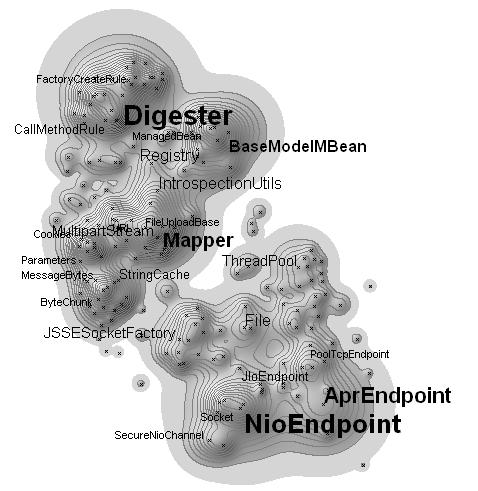
\includegraphics[width=\figwidth]{apache-tomcat-bw.png}\\
  Apache Tomcat
\end{center}
\end{minipage}~
\begin{minipage}{\figwidth}
\begin{center}
  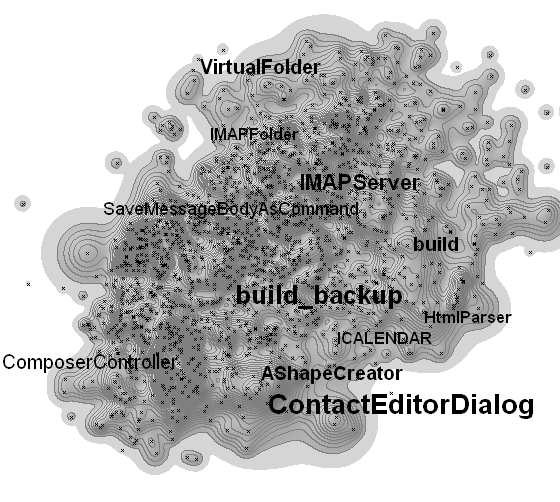
\includegraphics[width=\figwidth]{columba-bw.png}\\
  Columba
\end{center}
\end{minipage}
\begin{minipage}{\figwidth}
\begin{center}
  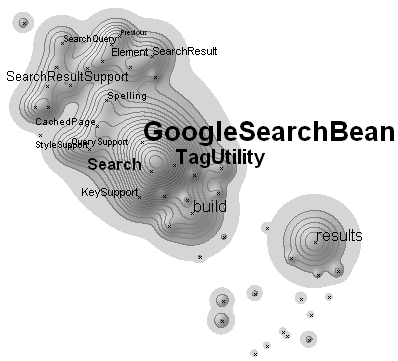
\includegraphics[width=\figwidth]{google-taglib-bw.png}\\
  Google Taglib
\end{center}
\end{minipage}
\begin{minipage}{\figwidth}
\begin{center}
  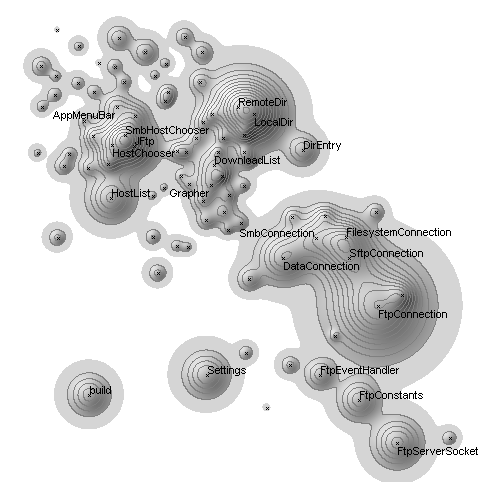
\includegraphics[width=\figwidth]{j-ftp-bw.png}\\
  JFtp
\end{center}
\end{minipage}
\begin{minipage}{\figwidth}
\begin{center}
  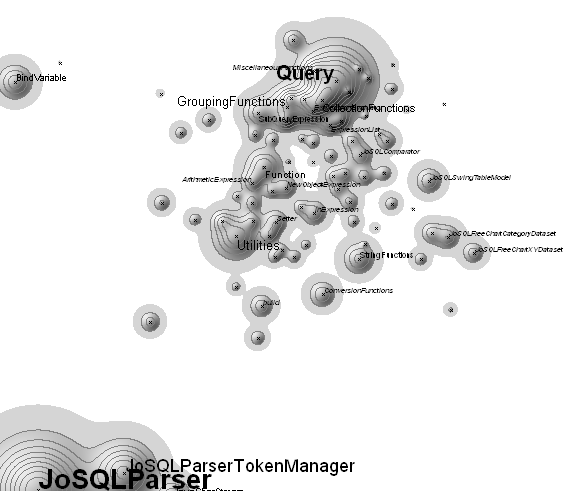
\includegraphics[width=\figwidth]{JoSQL-bw.png}\\
  JoSQL
\end{center}
\end{minipage}
\begin{minipage}{\figwidth}
\begin{center}
  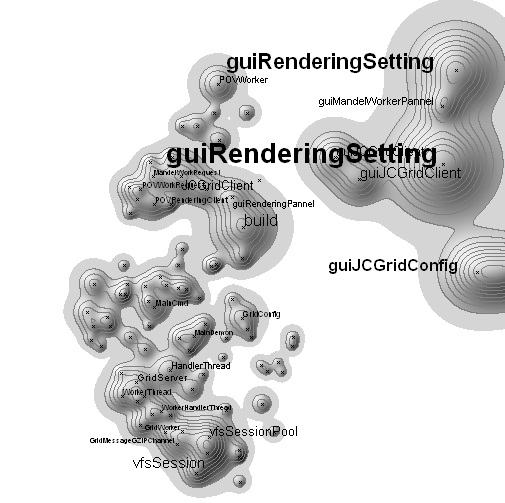
\includegraphics[width=\figwidth]{jcgrid-bw.png}\\
  JCGrid
\end{center}
\end{minipage}
\end{center}
\vspace{1ex}
    \caption{Overview of the software maps of six open source systems. Each map reveals a distinct spatial structure. When consequently applied to every visualization, the consistent layout may soon turn into the system's iconic fingerprint. An engineer might \eg point to the top left map and say: ``Look, this huge {\tt Digester} peninsula in the north, that must be Tomcat. I know it from last year's code review.''.
    }
    \label{fig:fullpage}
\end{figure*} 

% ~~~~~~~~~~~~~~~~~~~~~~~~~~~~~~~~~~~~~~~~~~~~~~~~~~~~~~~~~~~~~~~~~~~~~~~~~~~~~~
\subsection{Open-source examples}

We applied the \SOCA approach to all systems listed in the field study by Cabral and Marques \cite{Cabr07a}. They list 32 systems, including 4 of each type of application (Standalone, Server, Server Applications, Libraries) and selected programming language (Java, .NET).  

Figure \ref{fig:fullpage} shows the software map for six of these systems: Apache Tomcat, Columba, Google Taglib, JFtp, JCGrid and JoSQL. Each system reveals a distinct spatial structure. Some fall apart into many islands, like JFtp, whereas others cluster into one (or possibly two) large contents, like Columba and Apache Tomcat. The 36 case-studies raised interesting questions for future work regarding the correlation between a system's layout and code quality. For example, do large continents indicate bad modularizations? Or, do archipelagoes indicate low coupling?

%Each system's size in TLC and KLOC is listed in Table~\ref{tab:six}.

%\begin{table}[htdp]
%\begin{center}
%\begin{tabular}{l|rr}
%\textbf{System} & \textbf{\# Top-level} & \textbf{KLOC} \\
% & \textbf{classes} & \\
%\hline
%Apache Tomcat & 162 & 14'700 \\
%Columba & 1'549 & 53'500 \\
%Google Taglib & 20 & 940 \\ 
%JFtp & 78 & 3'470 \\
%JCGrid & 94 & 3'630 \\
%JoSQL & 83 & 6'480 \\
%\end{tabular}
%\end{center}
%\vspace{1ex}
%\caption{Statistics of the six systems in Figure~\ref{fig:fullpage}. \AK{Are you sure this is KLOC? Does Google Taglib really have 0.9 million(!) lines of code in 20 classes only?}
%}
%\label{tab:six}
%\end{table}

% ~~~~~~~~~~~~~~~~~~~~~~~~~~~~~~~~~~~~~~~~~~~~~~~~~~~~~~~~~~~~~~~~~~~~~~~~~~~~~~
\subsection{Thematic cartography examples}

\begin{figure}
\begin{center}
\begin{minipage}{1.4\figwidth}
\begin{center}
  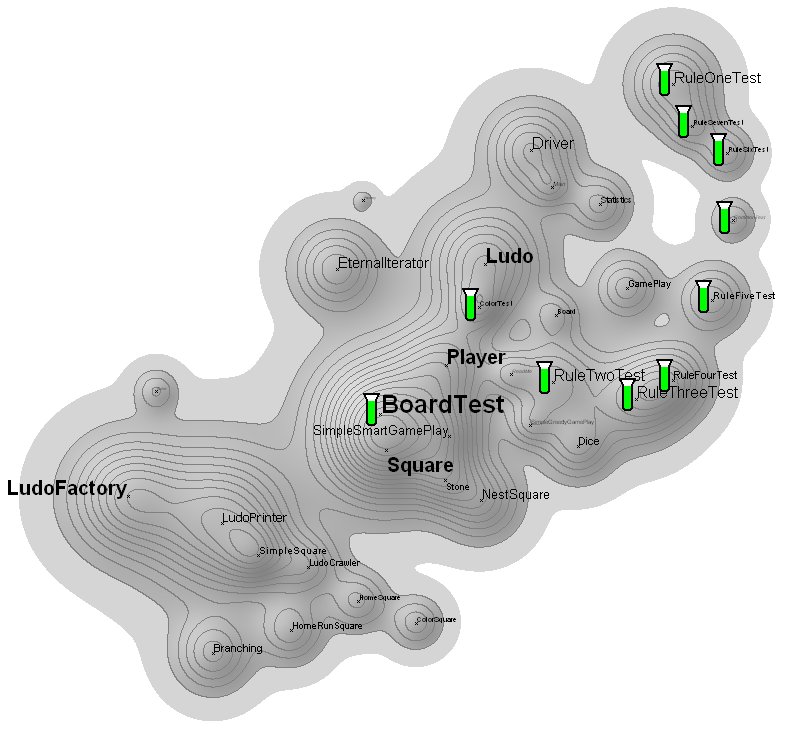
\includegraphics[width=1.4\figwidth]{ludo-v4-testtubes.png}
\end{center}
\end{minipage}
\begin{minipage}{1.4\figwidth}
\begin{center}
  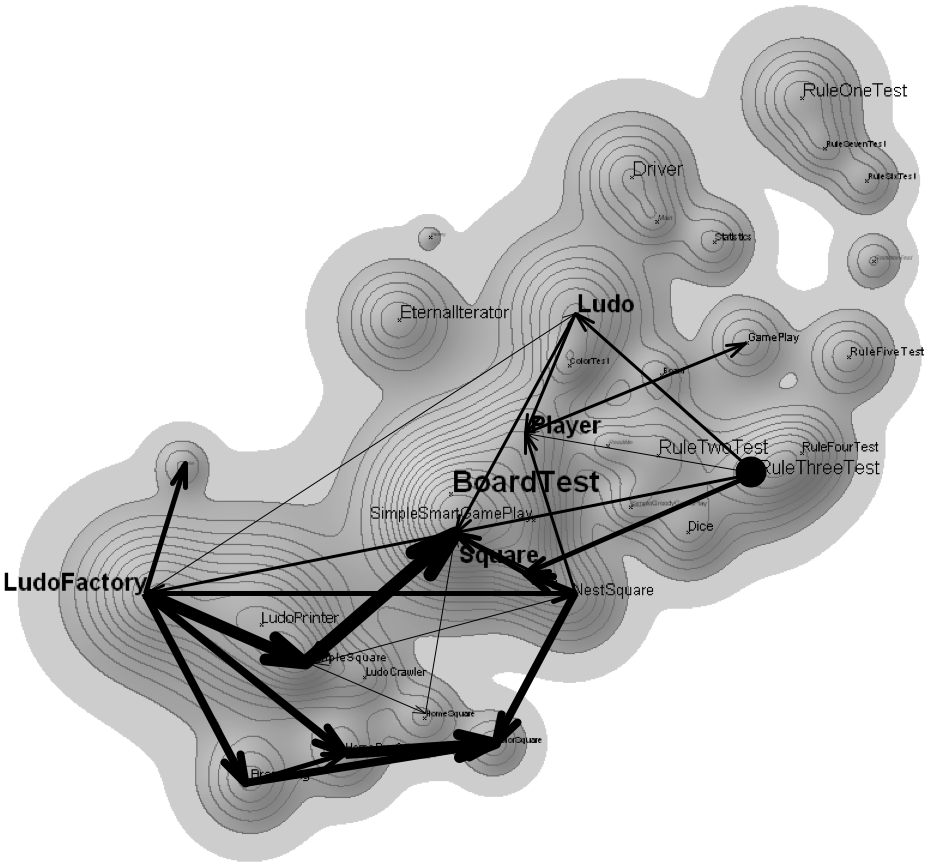
\includegraphics[width=1.4\figwidth]{ludo-v4-testexecution.png}
\end{center}
\end{minipage}
\end{center}
    \caption{Software maps with thematic overlay: (left) glyphs are drawn on top of the map, to display additional information. Each test tube glyph indicates the location of unit test case, (right) invocation edges are drawn on top of the map, showing the trace of executing the {\tt RuleThreeTest} test case.}
    \label{fig:mock}
\end{figure}

Software maps can be used as canvas for more specialized visualizations of the same system. In the following, we provide two thematic visualization of the Ludo system that might benefit from consistent layout. (The maps in this subsection are mockups, not yet fully supported by \TOOL.)

\begin{itemize}

\item Boccuzzo and Gall present a set of metaphors for the visual shape of entities \cite{Bocc07a}. They use simple and well-known graphical elements from daily life, such as houses and tables. However they use conventional albeit arbitrary layouts, where the distribution of glyphs often does not bear a meaningful interpretation. The first map in Figure~\ref{fig:mock} (on the left) employs their technique on top of a software map, using test tubes to indicate the distribution of test cases.

\item Greevy \etal present a three-dimensional variation of System Complexity View to visualize a System's dynamic runtime state \cite{Gree05d}. They connect classes with edges representing method invocation, and stack boxes on top of each other to represent a class's instances.
Since System Complexity Views do not capture any notion of position, the lengths of their invocation edges do not express any real sense of distance.

Figure~\ref{fig:mock} (on the right) employs their approach on top of a software map, drawing invocation edges in a two-dimensional plane.
Here the distances have an interpretation in terms of lexical distance, so the lengths of invocation edges are meaningful.
A short edge indicates that closely related artifacts are invoking each other, whereas long edges indicate a ``long-distance call'' to a lexically unrelated class.

\end{itemize}

